\pgfplotsset{compat=1.15}
	
\usetikzlibrary{arrows}
\definecolor{ffqqqq}{rgb}{1,0,0}
\definecolor{qqwuqq}{rgb}{0,0.39215686274509803,0}
\definecolor{qqqqff}{rgb}{0,0,1}
\definecolor{ududff}{rgb}{0.30196078431372547,0.30196078431372547,1}
\begin{figure}[h!]
    \centering
    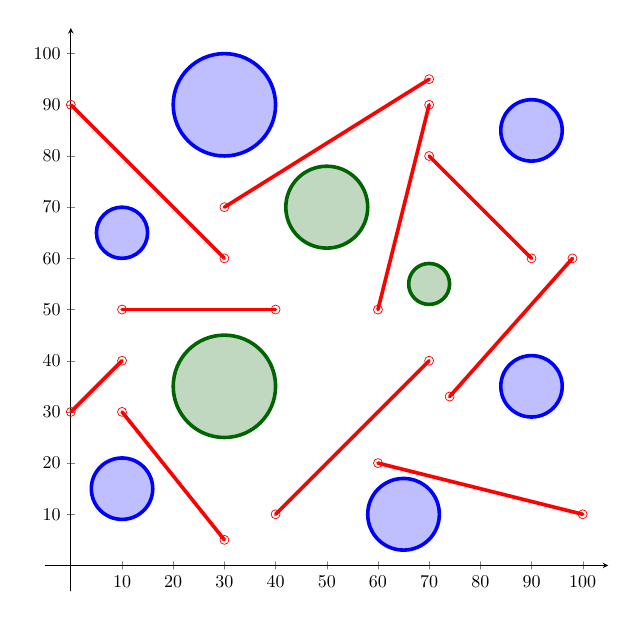
\begin{tikzpicture}[line cap=round,line join=round,>=triangle 45,x=0.1cm,y=0.1cm, scale = 0.65]
        \begin{axis}[
            x=0.1cm,y=0.1cm,
            axis lines=middle,
            xmin=-5,
            xmax=105,
            ymin=-5,
            ymax=105,
            xtick={0,10,...,100},
            ytick={0,10,...,100},]
            \draw [rotate around={0:(10,15)},line width=2pt,color=qqqqff,fill=qqqqff,fill opacity=0.25] (10,15) ellipse (0.6cm and 0.6cm);
            \draw [rotate around={0:(70,55)},line width=2pt,color=qqwuqq,fill=qqwuqq,fill opacity=0.25] (70,55) ellipse (0.4cm and 0.4cm);
            \draw [rotate around={0:(50,70)},line width=2pt,color=qqwuqq,fill=qqwuqq,fill opacity=0.25] (50,70) ellipse (0.8cm and 0.8cm);
            \draw [rotate around={0:(65,10)},line width=2pt,color=qqqqff,fill=qqqqff,fill opacity=0.25] (65,10) ellipse (0.7cm and 0.7cm);
            \draw [rotate around={0:(10,65)},line width=2pt,color=qqqqff,fill=qqqqff,fill opacity=0.25] (10,65) ellipse (0.5cm and 0.5cm);
            \draw [rotate around={0:(30,35)},line width=2pt,color=qqwuqq,fill=qqwuqq,fill opacity=0.25] (30,35) ellipse (1cm and 1cm);
            \draw [rotate around={0:(90,35)},line width=2pt,color=qqqqff,fill=qqqqff,fill opacity=0.25] (90,35) ellipse (0.6cm and 0.6cm);
            \draw [rotate around={0:(90,85)},line width=2pt,color=qqqqff,fill=qqqqff,fill opacity=0.25] (90,85) ellipse (0.6cm and 0.6cm);
            \draw [rotate around={0:(30,90)},line width=2pt,color=qqqqff,fill=qqqqff,fill opacity=0.25] (30,90) ellipse (1cm and 1cm);
            \draw [line width=2pt,color=ffqqqq] (0,90)-- (30,60);
            \draw [line width=2pt,color=ffqqqq] (40,50)-- (10,50);
            \draw [line width=2pt,color=ffqqqq] (0,30)-- (10,40);
            \draw [line width=2pt,color=ffqqqq] (10,30)-- (30,5);
            \draw [line width=2pt,color=ffqqqq] (40,10)-- (70,40);
            \draw [line width=2pt,color=ffqqqq] (60,20)-- (100,10);
            \draw [line width=2pt,color=ffqqqq] (30,70)-- (70,95);
            \draw [line width=2pt,color=ffqqqq] (70,90)-- (60,50);
            \draw [line width=2pt,color=ffqqqq] (70,80)-- (90,60);
            \draw [line width=2pt,color=ffqqqq] (74,33)-- (98,60);
            \begin{scriptsize}
                \draw [color=ffqqqq] (0,90) circle (2.5pt);
                \draw [color=ffqqqq] (30,60) circle (2.5pt);
                \draw [color=ffqqqq] (40,50) circle (2.5pt);
                \draw [color=ffqqqq] (10,50) circle (2.5pt);
                \draw [color=ffqqqq] (0,30) circle (2.5pt);
                \draw [color=ffqqqq] (10,40) circle (2.5pt);
                \draw [color=ffqqqq] (10,30) circle (2.5pt);
                \draw [color=ffqqqq] (30,5) circle (2.5pt);
                \draw [color=ffqqqq] (40,10) circle (2.5pt);
                \draw [color=ffqqqq] (70,40) circle (2.5pt);
                \draw [color=ffqqqq] (60,20) circle (2.5pt);
                \draw [color=ffqqqq] (100,10) circle (2.5pt);
                \draw [color=ffqqqq] (30,70) circle (2.5pt);
                \draw [color=ffqqqq] (70,95) circle (2.5pt);
                \draw [color=ffqqqq] (70,90) circle (2.5pt);
                \draw [color=ffqqqq] (60,50) circle (2.5pt);
                \draw [color=ffqqqq] (70,80) circle (2.5pt);
                \draw [color=ffqqqq] (90,60) circle (2.5pt);
                \draw [color=ffqqqq] (74,33) circle (2.5pt);
                \draw [color=ffqqqq] (98,60) circle (2.5pt);
            \end{scriptsize}
        \end{axis}
    \end{tikzpicture}
    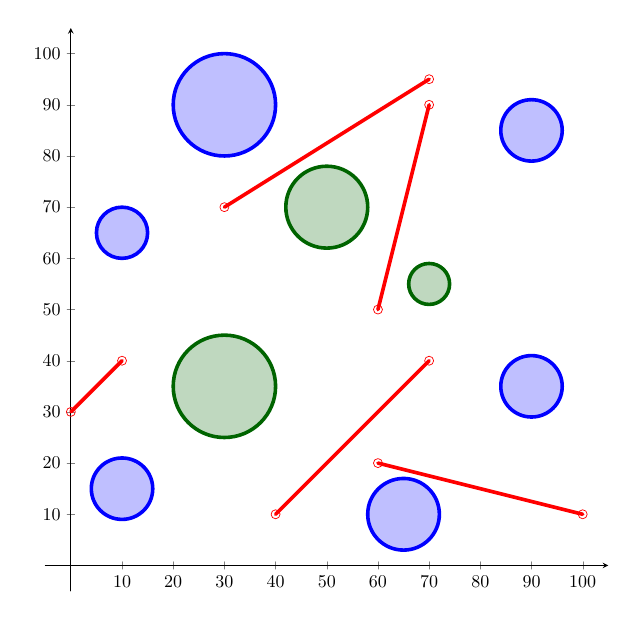
\begin{tikzpicture}[line cap=round,line join=round,>=triangle 45,x=0.1cm,y=0.1cm, scale = 0.65]
        \begin{axis}[
            x=0.1cm,y=0.1cm,
            axis lines=middle,
            xmin=-5,
            xmax=105,
            ymin=-5,
            ymax=105,
            xtick={0,10,...,100},
            ytick={0,10,...,100},]
            \draw [rotate around={0:(10,15)},line width=2pt,color=qqqqff,fill=qqqqff,fill opacity=0.25] (10,15) ellipse (0.6cm and 0.6cm);
            \draw [rotate around={0:(70,55)},line width=2pt,color=qqwuqq,fill=qqwuqq,fill opacity=0.25] (70,55) ellipse (0.4cm and 0.4cm);
            \draw [rotate around={0:(50,70)},line width=2pt,color=qqwuqq,fill=qqwuqq,fill opacity=0.25] (50,70) ellipse (0.8cm and 0.8cm);
            \draw [rotate around={0:(65,10)},line width=2pt,color=qqqqff,fill=qqqqff,fill opacity=0.25] (65,10) ellipse (0.7cm and 0.7cm);
            \draw [rotate around={0:(10,65)},line width=2pt,color=qqqqff,fill=qqqqff,fill opacity=0.25] (10,65) ellipse (0.5cm and 0.5cm);
            \draw [rotate around={0:(30,35)},line width=2pt,color=qqwuqq,fill=qqwuqq,fill opacity=0.25] (30,35) ellipse (1cm and 1cm);
            \draw [rotate around={0:(90,35)},line width=2pt,color=qqqqff,fill=qqqqff,fill opacity=0.25] (90,35) ellipse (0.6cm and 0.6cm);
            \draw [rotate around={0:(90,85)},line width=2pt,color=qqqqff,fill=qqqqff,fill opacity=0.25] (90,85) ellipse (0.6cm and 0.6cm);
            \draw [rotate around={0:(30,90)},line width=2pt,color=qqqqff,fill=qqqqff,fill opacity=0.25] (30,90) ellipse (1cm and 1cm);
            \draw [line width=2pt,color=ffqqqq] (0,30)-- (10,40);
            \draw [line width=2pt,color=ffqqqq] (40,10)-- (70,40);
            \draw [line width=2pt,color=ffqqqq] (60,20)-- (100,10);
            \draw [line width=2pt,color=ffqqqq] (30,70)-- (70,95);
            \draw [line width=2pt,color=ffqqqq] (70,90)-- (60,50);				
            \begin{scriptsize}
                \draw [color=ffqqqq] (0,30) circle (2.5pt);
                \draw [color=ffqqqq] (10,40) circle (2.5pt);
                \draw [color=ffqqqq] (40,10) circle (2.5pt);
                \draw [color=ffqqqq] (70,40) circle (2.5pt);
                \draw [color=ffqqqq] (60,20) circle (2.5pt);
                \draw [color=ffqqqq] (100,10) circle (2.5pt);
                \draw [color=ffqqqq] (30,70) circle (2.5pt);
                \draw [color=ffqqqq] (70,95) circle (2.5pt);
                \draw [color=ffqqqq] (70,90) circle (2.5pt);
                \draw [color=ffqqqq] (60,50) circle (2.5pt);
            \end{scriptsize}
        \end{axis}
    \end{tikzpicture}
    \caption{Problem data of the \KMPHN \ and \KMPN}
    \label{fig:initialdata}
\end{figure}